\scanpage{90}

que $(j,k\in J\text{ et }j\leq i\leq k)\Longrightarrow i\in J$. On dit aussi, \unsure{donc|alors}, que $J$ est une \uline{bande} de $I$, \uline{C}'est \deleted{\unsure{une propriété|une prop.|une top.}} \inserted{une} propriété sym. par passage de $I$ à $I^\circ$.
\inserted{Toute intersection de bandes est une bande. La plus petite bande contenant $J$ est $\deleted{\unsure{\bar J}\cap\widetilde J}$}
% Formula (84) runs obliquely up the left margin and is attached to the preceding inserted sentence by a brace-like leader.
\margin{$\displaystyle(84)\quad\underset{\substack{\Vert\,\mathrm{déf}\\B(J)}}{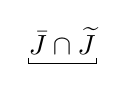
\begin{tikzpicture}[baseline=(term.base)]\node[inner sep=0pt] (term) {$\bar J\cap\widetilde J$};\draw ([yshift=-1pt]term.south west) -- ([yshift=-3pt]term.south west) -- ([yshift=-3pt]term.south east) -- ([yshift=-1pt]term.south east);\end{tikzpicture}}=\{i\in I\mid\exists j,k\in J\text{ tels que }j\leq i\leq k\}$}

Soient $J,K$ deux \deleted{\unsure{bandes}} \inserted{parties} de $I$, on écrit
\[
(85)\qquad J\prec K\quad\overset{\mathrm{déf}}{\Longleftrightarrow}\quad J\subset\bar K,\ K\subset\widetilde J
\]
(relation de \uline{domination}). C'est une relation de préordre sur l'ens $\mathcal P(I)$ des parties de $I$, la relation d'équivalence associée est
\[
(86)\qquad\begin{aligned}
J\sim K&\Longleftrightarrow J\subset\underset{B(K)}{
\begin{tikzpicture}[baseline=(term.base)]\node[inner sep=0pt] (term) {$\bar K\cap\widetilde K$};\draw ([yshift=-1pt]term.south west) -- ([yshift=-3pt]term.south west) -- ([yshift=-3pt]term.south east) -- ([yshift=-1pt]term.south east);\end{tikzpicture}},\ K\subset\underset{B(J)}{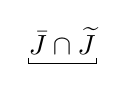
\begin{tikzpicture}[baseline=(term.base)]\node[inner sep=0pt] (term) {$\bar J\cap\widetilde J$};\draw ([yshift=-1pt]term.south west) -- ([yshift=-3pt]term.south west) -- ([yshift=-3pt]term.south east) -- ([yshift=-1pt]term.south east);\end{tikzpicture}}\\
&\Longleftrightarrow B(J)=B(K)
\end{aligned}
\]
L'ens ordonné quotient est l'ens des \uline{bandes} de $I$, ordonné par la relation de \deleted{\unsure{inclusion|l'inclusion}} \inserted{domination}.

Supposons maintenant que $J$ et $K$ soient des bandes, \inserted{\unsure{avec|on a} $J\prec K$,} soit $I'$ la bande engendrée par $J\cup K$, on a
\[
(87\unsure{)|]}\qquad\begin{aligned}
I'&=\{i\in I\mid\exists j\in J,k\in K\text{ t.q. }j\leq i\leq k\}\\
&=\widetilde J\cap\bar K
\end{aligned}
\]
et $J$ est fermé dans $I'$, $K$ est ouvert dans $I'$ enfin \deleted{\unsure{et|\ell|\xi}} $-\unsure{K|K\prime}$ est dense dans $I'$ et $J$ codense dans $I'$ i.e. $I'\unsure{=|\subset}\bar K$ et $I'\subset\widetilde J$ \deleted{\unsure{et|donc}} i.e. $I'\subset\bar K\cap\widetilde J$ (on a $=$ égalité!). Inversement si $\exists$ bande $I'$ tel que $J$ soit un fermé codense dans $I'$, $K$ un ouvert dense dans $I'$, alors $J$ et $K$ sont des bandes, $J\prec K$, et ainsi, $I'=\widetilde J\cap\bar K$.
\margin{89}
